\documentclass[12pt, a4paper]{article}

\usepackage{lastpage}
\usepackage{mathtools}
\usepackage{xltxtra}
\usepackage{libertine}
\usepackage{amsmath}
\usepackage{amsthm}
\usepackage{amsfonts}
\usepackage{amssymb}
\usepackage{enumitem}
\usepackage{xcolor}
\usepackage[left=1.5cm, right=1.5cm, top=2cm, bottom=2cm, bindingoffset=0cm, headheight=15pt]{geometry}
\usepackage{fancyhdr}
\usepackage[russian]{babel}
% \usepackage[utf8]{inputenc}
\usepackage{catchfilebetweentags}
\usepackage{accents}
\usepackage{calc}
\usepackage{etoolbox}
\usepackage{mathrsfs}
\usepackage{wrapfig}

\providetoggle{useproofs}
\settoggle{useproofs}{false}

\pagestyle{fancy}
\lfoot{M3137y2019}
\rhead{\thepage\ из \pageref{LastPage}}

\newcommand{\R}{\mathbb{R}}
\newcommand{\Q}{\mathbb{Q}}
\newcommand{\C}{\mathbb{C}}
\newcommand{\Z}{\mathbb{Z}}
\newcommand{\B}{\mathbb{B}}
\newcommand{\N}{\mathbb{N}}

\newcommand{\const}{\text{const}}

\newcommand{\teormin}{\textcolor{red}{!}\ }

\DeclareMathOperator*{\xor}{\oplus}
\DeclareMathOperator*{\equ}{\sim}
\DeclareMathOperator{\Ln}{\text{Ln}}
\DeclareMathOperator{\sign}{\text{sign}}
\DeclareMathOperator{\Sym}{\text{Sym}}
\DeclareMathOperator{\Asym}{\text{Asym}}
% \DeclareMathOperator{\sh}{\text{sh}}
% \DeclareMathOperator{\tg}{\text{tg}}
% \DeclareMathOperator{\arctg}{\text{arctg}}
% \DeclareMathOperator{\ch}{\text{ch}}

\DeclarePairedDelimiter{\ceil}{\lceil}{\rceil}
\DeclarePairedDelimiter{\abs}{\left\lvert}{\right\rvert}

\setmainfont{Linux Libertine}

\theoremstyle{plain}
\newtheorem{axiom}{Аксиома}
\newtheorem{lemma}{Лемма}

\theoremstyle{remark}
\newtheorem*{remark}{Примечание}
\newtheorem*{exercise}{Упражнение}
\newtheorem*{consequence}{Следствие}
\newtheorem*{example}{Пример}
\newtheorem*{observation}{Наблюдение}

\theoremstyle{definition}
\newtheorem{theorem}{Теорема}
\newtheorem*{definition}{Определение}
\newtheorem*{obozn}{Обозначение}

\setlength{\parindent}{0pt}

\newcommand{\dbltilde}[1]{\accentset{\approx}{#1}}
\newcommand{\intt}{\int\!}

% magical thing that fixes paragraphs
\makeatletter
\patchcmd{\CatchFBT@Fin@l}{\endlinechar\m@ne}{}
  {}{\typeout{Unsuccessful patch!}}
\makeatother

\newcommand{\get}[2]{
    \ExecuteMetaData[#1]{#2}
}

\newcommand{\getproof}[2]{
    \iftoggle{useproofs}{\ExecuteMetaData[#1]{#2proof}}{}
}

\newcommand{\getwithproof}[2]{
    \get{#1}{#2}
    \getproof{#1}{#2}
}

\newcommand{\import}[3]{
    \subsection{#1}
    \getwithproof{#2}{#3}
}

\newcommand{\given}[1]{
    Дано выше. (\ref{#1}, стр. \pageref{#1})
}

\renewcommand{\ker}{\text{Ker }}
\newcommand{\im}{\text{Im }}
\newcommand{\grad}{\text{grad}}

\lhead{Дискретная математика}
\cfoot{}
\rfoot{Лекция 8}

\begin{document}

\section*{НКА}

Уберем ограничение на единственность перехода по символу, тогда получим \textbf{недетерменированный КА}:

\begin{figure}[h]
    \centering
    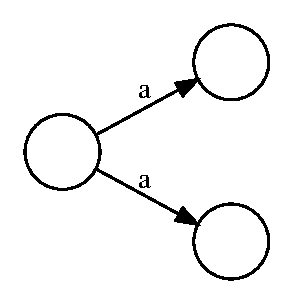
\includegraphics{graphs/8.1.dot.eps}
\end{figure}

Кроме того, уберем ограничение на существование перехода, тогда если перехода нет, то слово не допускается в искомый язык.
Слово допускается, если существует последовательность недетерменированных выборов, приводящая к допуску.

\begin{example}
    Автомат для слов с суффиксом $010$:
    \begin{figure}[h]
        \centering
        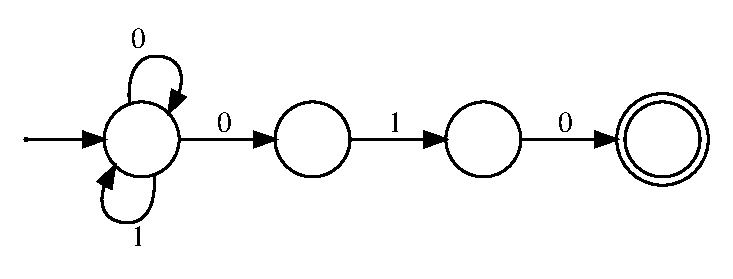
\includegraphics{graphs/8.2.dot.eps}
    \end{figure}
\end{example}

\subsection*{Алгоритм проверки допуска НКА}

$Q=\{1, 2\ldots q\}$ --- все вершины

\texttt{term} --- массив булевых переменных терминальности состояний.

\texttt{go[c][i]} --- вектор вершин, в которые можно попасть из вершины \texttt{i} по символу \texttt{c}

Построим динамику \texttt{can[i][u]} --- можно ли за $i$ шагов попасть в состояние $u$.

\begin{verbatim}
accept(x)
    can[0][s] = true
    for i = 0...len(x) - 1
        c = x[i]
        for u = 1...q
            if (can[i][u])
                for v : go[u][c]
                    can[i + 1][v] = true
    for u = 1...q
        if (can[len(x)][u] and term[u])
            return true
    return false
\end{verbatim}

Применим для автомата слов с суффиксом $010$ и слова $01010$:
$$\begin{array}{c|cccc}
          & 1 & 2 & 3 & 4      \\
        \hline
        0 & +                  \\
        1 & + & +              \\
        2 & + &   & +          \\
        3 & + & + &   & +      \\
        4 & + &   & +          \\
        5 & + & + &   & \oplus
    \end{array}$$
Заметим, что 2 строка = 4 строка и 3 символ равен 5 символу, поэтому 3 строка = 5 строка.

Построим по этой динамике ДКА с булевыми векторами строк в вершинах.

\begin{verbatim}
ds = 1 << s
for du = 0...2**q-1
    for c - symbol
        dv = 0
        for u = 0...q-1
            if (du & (1 << u)) != 0
                for v : go[u][c]
                    dv |= (1 << v)
        dgo[du][c] = dv
    if (du & term != 0)
        dterm[du] = true
\end{verbatim}

Для ускорения можно перебирать не все маски, а только те, которые встретились, т.е. DFS/BFS. Без этого $\mathcal O(2^q\cdot poly(q, \sigma))$, с оптимизацией $\mathcal O(ans\cdot poly(q, \sigma)), ans=$ число состояний ДКА.

Таким образом, мы по любому НКА можем построить ДКА с таким же языков, т.е. выполнятся следующее:
\begin{theorem}
    $\forall$ НКА $A$ $\exists$ ДКА $A_D : L(A) = L(A_D)$
\end{theorem}

Создадим в НКА ребра, по которым можно перейти, не считав символа, и будем обозначать такое ребро $\varepsilon$. Эта конструкция называется \textbf{$\varepsilon$-НКА}.

Докажем, что $\varepsilon$-НКА эквивалентен ДКА построением:

\begin{enumerate}
    \item Построим граф $\varepsilon$-переходов и создадим его транзитивное замыкание. Добавленные замыканием ребра добавим в исходный автомат. Язык автомата от этого не изменился, т.к. переход по новому ребру эквивалентен $n$ переходов по $\varepsilon$-ребрам в исходном графе. Теперь можно не делать два $\varepsilon$-перехода подряд.
    \item Если из обычной вершины есть $\varepsilon$-переход в терминальную вершину, то сделаем эту вершину терминальной. Язык автомата от этого преобразования не изменился. Теперь последний переход происходит не по $\varepsilon$.

          \pagebreak

    \item Преобразуем \begin{figure}[h]
              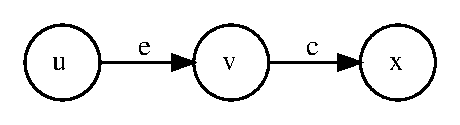
\includegraphics{graphs/8.3.dot.eps}
          \end{figure}

          в

          \begin{figure}[h]
              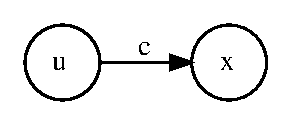
\includegraphics{graphs/8.4.dot.eps}
          \end{figure}

          Теперь можно не делать $\varepsilon$-переходы.

    \item Удалим $\varepsilon$-переходы.
\end{enumerate}

\begin{theorem}
    Клини.

    $$L \text{ --- регулярный} \Leftrightarrow \exists \text{ ДКА } A : L = L(A)$$
\end{theorem}
Докажем ``$\Rightarrow$''
\begin{figure}[h]
    \centering
    \begin{minipage}{.3\textwidth}
        \centering
        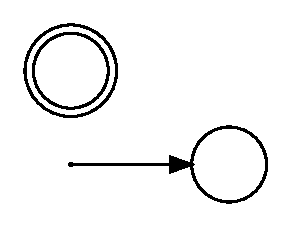
\includegraphics[scale=0.7]{graphs/8.5.dot.eps}
        \caption{Автомат для $\{\emptyset\}$}
    \end{minipage}%
    \begin{minipage}{.3\textwidth}
        \centering
        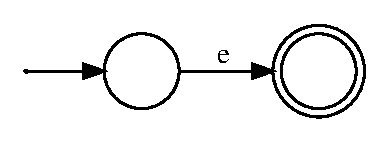
\includegraphics[scale=0.7]{graphs/8.6.dot.eps}
        \caption{Автомат $\{\varepsilon\}$}
    \end{minipage}
    \begin{minipage}{.3\textwidth}
        \centering
        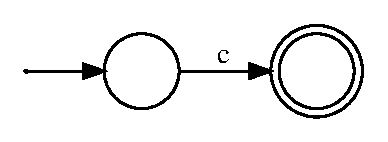
\includegraphics[scale=0.7]{graphs/8.7.dot.eps}
        \caption{Автомат $\{c\}$}
    \end{minipage}
    \begin{minipage}{.5\textwidth}
        \centering
        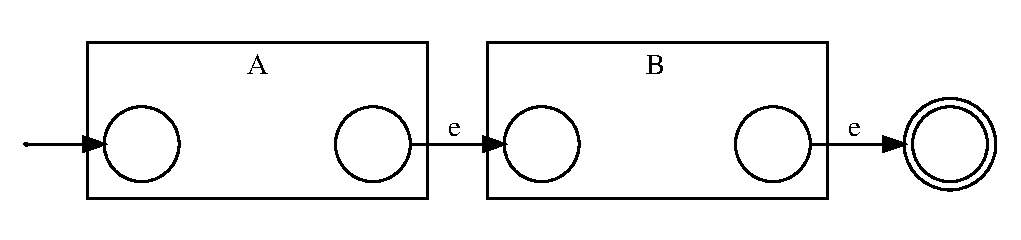
\includegraphics[scale=0.55]{graphs/8.8.dot.eps}
        \caption{Автомат $AB$}
    \end{minipage}%
    \begin{minipage}{.5\textwidth}
        \centering
        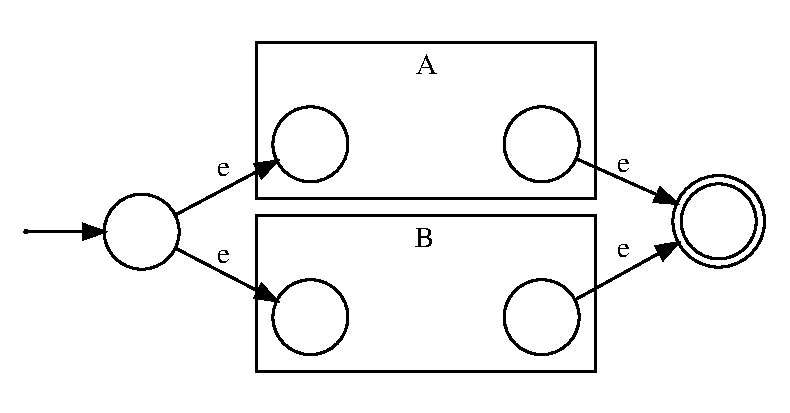
\includegraphics[scale=0.55]{graphs/8.9.dot.eps}
        \caption{Автомат $A\cup B$}
    \end{minipage}
    \begin{minipage}{.5\textwidth}
        \centering
        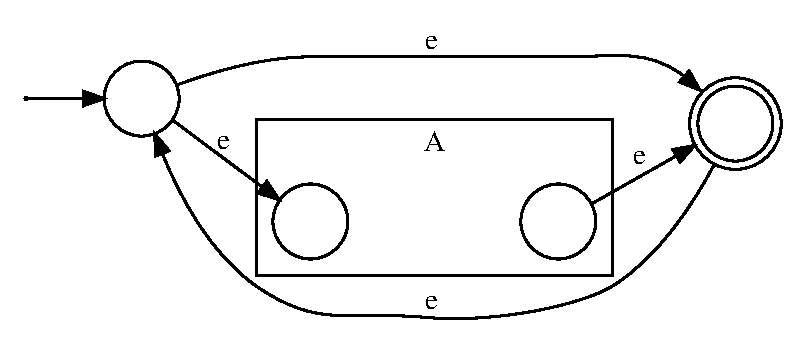
\includegraphics[scale=0.6]{graphs/8.10.dot.eps}
        \caption{Автомат $A^*$}
    \end{minipage}
\end{figure}

Докажем ``$\Leftarrow$''.
\begin{proof}
    $Q:=\{1,2,\ldots q\}$

    Построим $\sim q^3$ регулярных выражений, занумеруем их как $\xi_{ijk}, i=1\ldots q, j=1\ldots q, k = 0\ldots q$.

    $\xi_{ijk}$ задает слова, переводящие автомат из состояния $i$ в $j$, используя промежуточные состояния с номерами $\leq k$

    $\sphericalangle k=0, i=j, \xi_{ii0}=\varepsilon|c_1|c_2|\ldots$ --- из $i$ в $i$ без промежуточных состояний, т.к. состояний $\leq 0 \nexists$. $c_i$ --- петли в $i$.

    $\xi_{ij0}=c_1|c_2|\ldots$, $c_i$ --- переход $i\to j$

    $\xi_{ijk+1}=\xi_{ijk}|\xi_{ik+1k}(\xi_{k+1k+1k})^*\xi_{k+1jk}$ --- можем либо идти по пути с промежуточными $\leq k$, либо дойти $i\to k+1$, после чего $n\geq 0$ раз пройти $k+1\to k+1$ с промежуточными $\leq k$, после чего дойти $k+1\to j$  с промежуточными $k$ ($k$, а не $k+1$, т.к. номера состояний уникальны, а в $k+1$ мы уже не заходим)
\end{proof}

\end{document}